\section{Use Case Symbols and Notation's}
\vspace{0.2cm}

\textbf{Actor:} Represents a user or external system interacting with the system.\\
\textbf{Use Case:} Represents a specific functionality or task provided by the system.\\
\textbf{Association:} Shows the association between an actor and a use case.\\
\textbf{Generalization/Inheritance:} Indicates specialization and inheritance between use cases or actors.\\
\textbf{Include:} Represents the inclusion of one use case within another.\\
\textbf{Extend:} Indicates an extension of one use case by another.\\
These symbols simplify the representation of interactions and relationships in a use case diagram.\\
\begin{figure}[ht]
    \centering   
    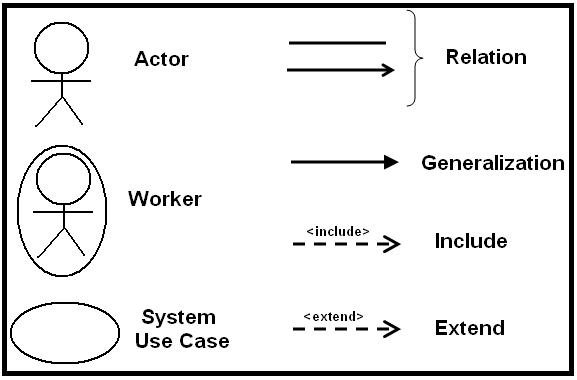
\includegraphics[width=\textwidth, height=8cm]{usecasediagram/Symbols-of-UML-Use-Case-diagram.jpg}
    \caption{Use Case Notation and Symbols}
    \label{fig:4.7}
\end{figure}